% !TEX root = ../main.tex

\chapter{Measurements}
\label{ch:measurements}
This work started from the existing SOSD benchmark going into the idea of implementing a learned index structure over the network in P4 and so far coming to a very theoretical result. The goal of this chapter is to try to get at least closer to understanding how much the ideas presented in the previous chapters could potentially benefit a concrete setup and implementation in the real world. As already quite extensively stated in section \ref{sect:rmionbmv2:evaluation} the P4 implementation as is cannot be tested on real world hardware. With this in mind the first section of this chapter will explain the choosen approach to still try to measure something useful in order to evaluate the potential impact. Further section \ref{sect:measurements:results} will present the measured results on the test university machine and finally the last section of this chapter will once again try to put the measured results into relation and give an evaluation.

\section{Method}
As already stated multiple times the following methods was choosen since not being able to actually run the generated P4 code on some concrete hardware due to multiple reasons also already described previously. In order to come up with some alternative we started with the idea that instead of actually measuring lookup time on concrete network hardware we could instead measure pure lookup time in an existing implementation and go on from there taking what we measured as maximally possible speedup. This immediately leads to the already established separation between pure lookup operation time and finally time spent for the last mile search. For this having a working benchmark implemented in C++ that can precisely measure the time it takes for a specific amount of lookups including last mile search on a dataset comes in handy. In order to measure hypothetical maximal time gain it is enough to separate the last mile search and measure only pure lookup time. The final piece to the puzzle now is that we have to assume that our network switches are able to process packets at a higher or at least a similar rate than a processor can handle pure lookup operations. This initially seemed like a bold claim to me but when taking into account that the proposed RMI implementation in P4 can easily scale horizontally with the amount of network hardware available, which is often available anyways, this quickly becomes realistic. Finally if we wanted to look at a closed system and effectively evaluate which method is faster, we would have to consider round trip time of packets. Although since not even being able to reliably test any of the implementation on actual hardware, this major concern for a real world setup is neglected in the scope of this work in the sense that we assume an application where packets need to travel over the network and with that over an RMI capable switch anyways and with that travel time spent is not really lost but instead used more efficiently.

\section{Results}
\label{sect:measurements:results}
In order to perform these measures we adapted the existing SOSD benchmark to measure not only lookup time and last mile search times at the same time but instead differenciate between the two steps and measuring only one at a time. The initial result though, when measuring only pure lookup operation time, is very disappointing. As shown in figure \ref{fig:books_200M_uint32-no-cc-mf} only a very small amount of time is spent on performing the pure RMI lookup operations.

\begin{figure}[!h]
  \centering
  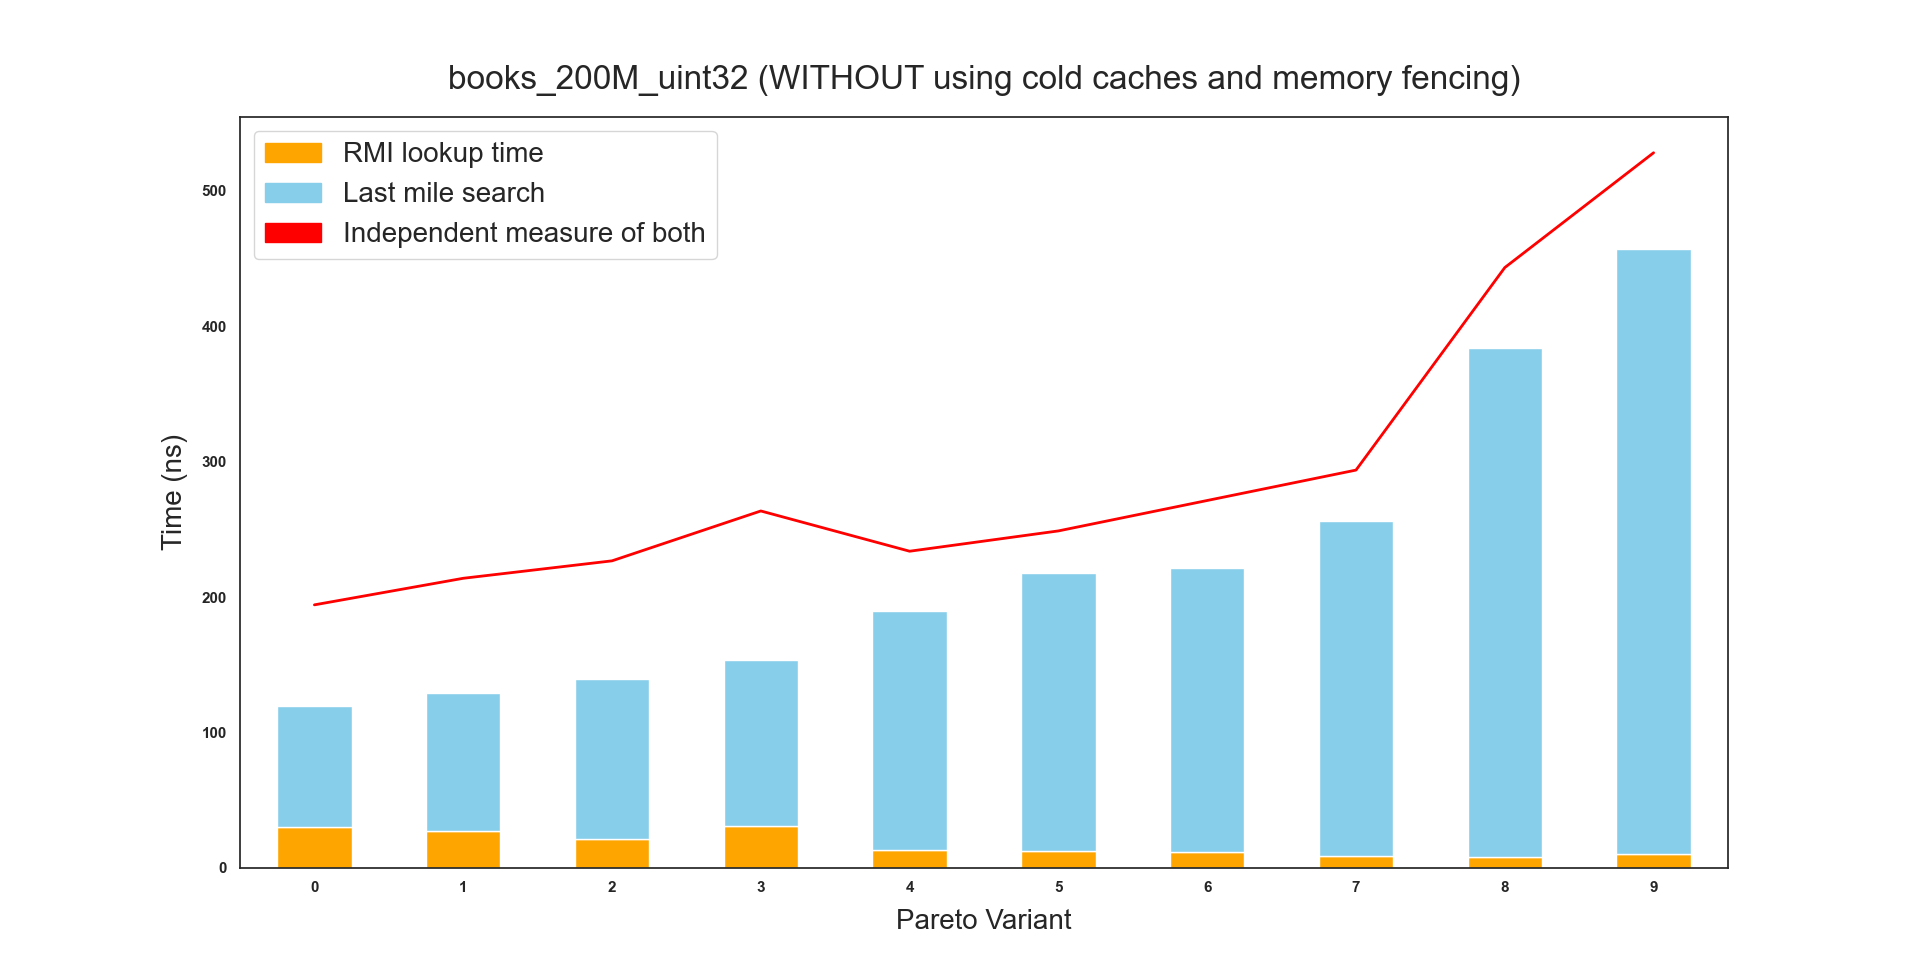
\includegraphics[width=1\textwidth]{measurements/books_200M_uint32-no-cc-mf}
  \caption[Pure lookup and last mile search time measures]{
    Running the SOSD benchmark on the books\_200M\_uint32 dataset differentiating between pure lookup time and last mile search time \emph{without using} cold caches or memory fencing.
  }
  \label{fig:books_200M_uint32-no-cc-mf}
\end{figure}

There are reasons for the way these measurements turned out which were already pointed out in \cite{sosd-neurips} in chapter 4.4. Namely these reasons are that lookups in a tight loop can greatly benefit from low level CPU optimization techniques like operator reordering or caching. The same applies for the above measurement in an even more intense way, since only measuring performance of essentially lots of tightly repeated FMA instructions which the processor will optimize into a more optimal instruction order and therefore exaggerate the measured performance of RMI. The same holds true for caching, in the sense that some of the requested data will already be loaded in some cache level and therefore access time is greatly reduced. Luckily though the authors of \cite{sosd-neurips} suggest and also already implemented a way to mitigate these usually very desired optimizations in the SOSD benchmark. The two proposed techniques are simple and aim at starting from a constant CPU state before every lookup calculation. The first technique called cold caching mitigates cache side effects by filling the L3 CPU cache with a constant randomly generated set of numbers before each lookup. The second technique called memory fencing aims at mitigating instruction reordering by introducing memory fences before each lookup using the appropriate Intel CPU instruction. With these techniques now in place running SOSD takes a lot longer and RMI performance drastically decreases but with the advantage that now more reliable meaures can be taken. The results from running the SOSD benchmark on the same dataset as previously but now using cold caches and memory fencing are shown in figure \ref{fig:books_200M_uint32}.

\begin{figure}[ht]
  \centering
  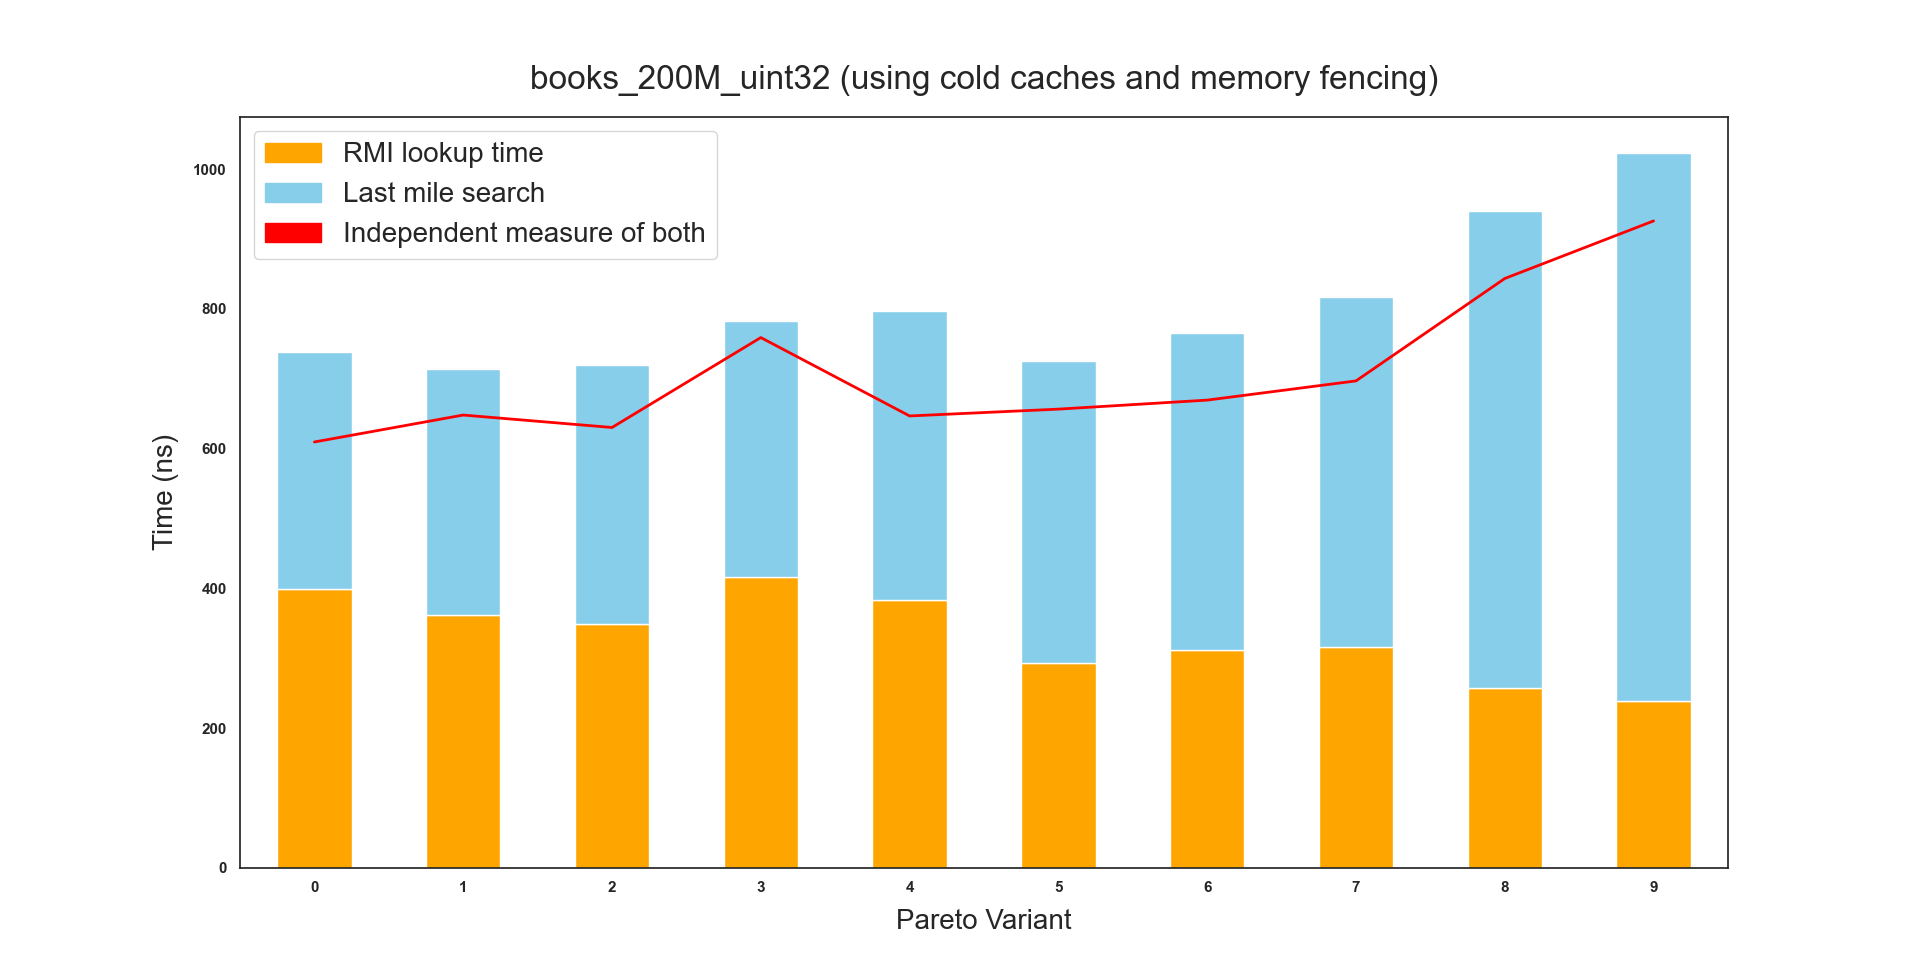
\includegraphics[width=1\textwidth]{measurements/books_200M_uint32}
  \caption[Lookup and last mile search time measures using cold caches and memory fencing]{
    Running the SOSD benchmark on the books\_200M\_uint32 dataset differentiating between pure lookup time and last mile search time \emph{using} cold caches and memory fencing.
  }
  \label{fig:books_200M_uint32}
\end{figure}

Further very similar observations can be made for the remaing 64-bit datasets all shown in the appendix in section \ref{sect:appendix:measurements}.

\section{Evaluation}
% Talk about ...
%
% obviously the blue bar (last mile search time) increases with larger pareto variant since in this configuration the reference implementation tries to reduce memory and therefore the average size of the last mile search interval increases
%
% the fact that we have less low level CPU optimization stuff like cache or instruciton reordering on switches
%
% the fact that under ideal conditions (travel time here anyways + implementation feasible in realistic stages + 64-bit base operations available on switch (which is A LOT not here yet)) we could potentially save time by outsource the RMI lookup operations to the switch.
